\subsection{UC28 - Suddivisione Planimetria}
\begin{figure}[H]
  \centering
  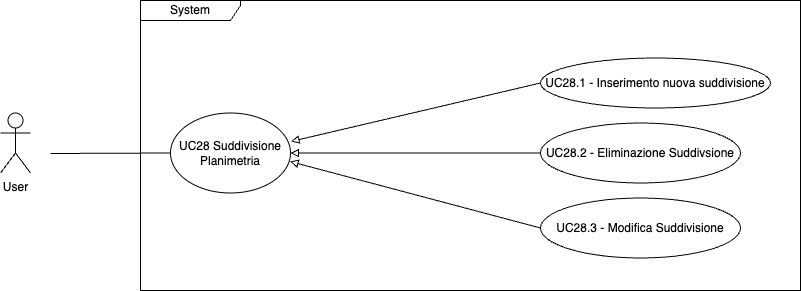
\includegraphics[width=0.8\textwidth]{UC_diagrams_21-27/UC28.drawio.png}
  \caption{Diagramma UML UC28 - Suddivisione Planimetria}
\end{figure}
\begin{itemize}
    \item \textbf{Attori:} User.
    \item \textbf{Pre-condizione:}  Il sistema é istanziato correttamente.
    \item \textbf{Post-condizione:} L'utente ha effettuato una modifica alla suddivisione del magazzino.
    \item \textbf{Scenario Principale:} L'utente entra nella schermata di suddivisione della planimetria e sceglie un'azione da compiere tra: Inserimento nuova suddivisione [UC28.1], Eliminazione suddivisione [UC28.2] e Modifica Suddivisione[UC28.3]. Le suddivisioni dividono il magazzino in zone adibite ad uno scopo evidenziandone la diversitá nell'ambiente 3D.
    \item \textbf{Generalizzazioni:} Sono presenti 3 Generalizzazioni:
        \begin{itemize}
        \item UC28.1 Inserimento nuova Suddivisone
        \item UC28 Eliminazione Suddivisione
        \item UC28.3 Modifica Suddivisione
    \end{itemize}
    \item \textbf{Estensioni:} -
\end{itemize}

\subsection{UC28.1 - Inserimento nuova suddivisione}
\begin{figure}[H]
  \centering
  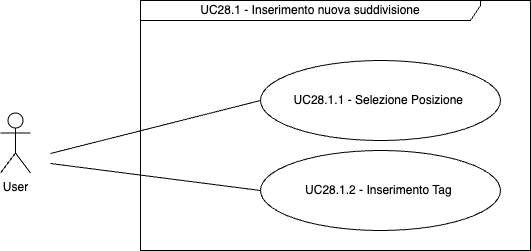
\includegraphics[width=0.8\textwidth]{UC_diagrams_21-27/UC28.1.drawio.png}
  \caption{Diagramma UML UC28.1 - Inserimento nuova suddivisione}
\end{figure}
\begin{itemize}
    \item \textbf{Attori:} User.
    \item \textbf{Pre-condizione:}  Il sistema é istanziato correttamente. L'utente ha scelto di inserire una nuova suddivisione della planimetria.
    \item \textbf{Post-condizione:} L'utente ha inserito correttamente una nuova suddivisione o ha annullato l'operazione.
    \item \textbf{Scenario Principale:} L'utente crea una nuova suddivisione scegliendone dapprima la posizione [UC28.1.1] e poi il tag [UC28.1.2]
    \item \textbf{Generalizzazioni:} -
    \item \textbf{Estensioni:} -
\end{itemize}

\subsection{UC28.1.1 - Selezione Posizione}
\begin{itemize}
    \item \textbf{Attori:} User.
    \item \textbf{Pre-condizione:}  L'utente è nella schermata di inserimento di una nuova suddivisione.
    \item \textbf{Post-condizione:} L'utente ha inserito la posizione della nuova suddivisione.
    \item \textbf{Scenario Principale:} L'utente sceglie una posizione per la nuova suddivisione all'interno della planimetria.
    \item \textbf{Estensioni:} -
\end{itemize}

\subsection{UC28.1.2 - Inserimento Tag}
\begin{itemize}
    \item \textbf{Attori:} User.
    \item \textbf{Pre-condizione:}  L'utente ha scelto una posizione per la nuova suddivisione.
    \item \textbf{Post-condizione:} L'utente ha inserito corretamente un Tag.
    \item \textbf{Scenario Principale:} L'utente sceglie un nome per la nuova suddivisione.
    \item \textbf{Generalizzazioni:} -
    \item \textbf{Estensioni:} -
\end{itemize}

\subsection{UC28.2 - Eliminazione suddivisione}
\begin{itemize}
    \item \textbf{Attori:} User.
    \item \textbf{Pre-condizione:}  L'utente è nella schermata di suddivisione planimetria.
    \item \textbf{Post-condizione:} L'utente ha eliminato una suddivisione o ha annullato.
    \item \textbf{Scenario Principale:} L'utente selezione una suddivisione e la elimina, oppure annulla il processo.
    \item \textbf{Generalizzazioni:} -
    \item \textbf{Estensioni:} -
\end{itemize}

\subsection{UC28.3 - Modifica suddivisione}
\begin{figure}[H]
  \centering
  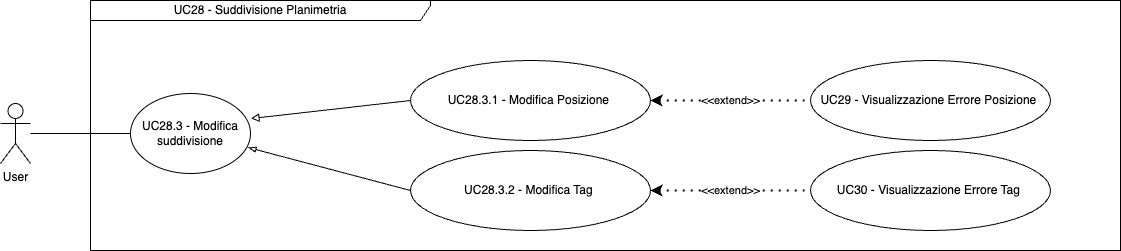
\includegraphics[width=0.8\textwidth]{UC_diagrams_21-27/UC28.3.drawio.png}
  \caption{Diagramma UML UC28.3 - Modifica suddivisione}
\end{figure}
\begin{itemize}
    \item \textbf{Attori:} User.
    \item \textbf{Pre-condizione:}  Il sistema é istanziato correttamente. L'utente ha scelto di modificare una suddivisione della planimetria.
    \item \textbf{Post-condizione:} L'utente ha modificato correttamente una nuova suddivisione o ha annullato l'operazione.
    \item \textbf{Scenario Principale:} L'utente modifica la posizione [UC28.3.1] o il tag [28.3.2] di una suddivisione
    \item \textbf{Generalizzazioni:} Sono presenti due generalizzazioni:
    \begin{itemize}
        \item UC28.3.1 Modifica Posizione
        \item UC28.3.2 Modifica Tag
    \end{itemize}
    \item \textbf{Estensioni:} -
\end{itemize}

\subsection{UC28.1.1 - Modifica Posizione}
\begin{itemize}
    \item \textbf{Attori:} User.
    \item \textbf{Pre-condizione:}  L'utente è nella schermata di modifica di una  suddivisione.
    \item \textbf{Post-condizione:} L'utente ha modifica la posizione della suddivisione.
    \item \textbf{Scenario Principale:} L'utente sceglie una nuova posizione per la suddivisione all'interno della planimetria.
    \item \textbf{Estensioni:} -
\end{itemize}

\subsection{UC28.1.2 - Modifica Tag}
\begin{itemize}
    \item \textbf{Attori:} User.
    \item \textbf{Pre-condizione:}  L'utente è nella schermata di modifica di una  suddivisione.
    \item \textbf{Post-condizione:} L'utente ha inserito corretamente un nuovo Tag.
    \item \textbf{Scenario Principale:} L'utente sceglie un nuovo nome per la suddivisione.
    \item \textbf{Generalizzazioni:} -
    \item \textbf{Estensioni:} -
\end{itemize}

